\documentclass[10pt]{article}
\usepackage{tmlr}
\usepackage{amsmath,amssymb}
\usepackage{booktabs,tabularx,array}
\usepackage{graphicx}
\usepackage{microtype}
\usepackage{tikz}
\usetikzlibrary{arrows.meta,positioning,shapes.misc}
\usepackage[hidelinks,pdfborder={0 0 0}]{hyperref}
\usepackage{url}
\newcolumntype{Y}{>{\raggedright\arraybackslash}X}
\newcommand{\yes}{\textbf{aligned}}
\newcommand{\no}{\textbf{misaligned}}

\title{Prospective measurement of decisions on unresolved scientific questions:
a three-question dual-instrument case series\thanks{Language-model systems assisted with research-agent execution and manuscript drafting and editing. They are not authors. The human authors verified the evidence, claims, citations and final text and retain full responsibility for the work.}}
\author{Anonymous Authors}
\date{}

\begin{document}
\maketitle

\begin{abstract}
Research-agent evaluations usually assume that a correct answer or reward is available when an agent acts. Live research creates a different measurement problem: a system must diagnose what is responsible for an unresolved result and choose the next discriminating experiment before the resolving evidence exists. We study a prospective contract for that setting. For each scientific question, a tool-capable host instrument and a typed deterministic controller receive the same frozen evidence state, record a diagnosis and an experiment choice separately, and cannot use the later scientific outcome. Agreement is recorded as an observation, not as a score. Later science is then bound to the frozen question and scores diagnosis and experiment choice independently.

The contract was executed on three valid questions in one quantum-compilation research programme. In the first two cases, both instruments agreed and both coordinates were aligned with the later evidence. In the third, both instruments agreed that a boundary predicate would change under an objective reweighting and both chose a complete census. The later exhaustive census covered 729 one-object and 38,760 two-object cases, 39,489 in total, and found zero predicate--label mismatches. Under the predeclared map, both diagnoses were therefore misaligned while both experiment choices remained aligned. Two earlier candidate questions were retained as contaminated because outcome-oriented surfaces became visible before instrument freeze. Two known malformed-success and recovery defects were also retained as fail-closed instrument limitations and were not repaired between cases. We report every case row by row and estimate no agreement rate, reliability, calibration, population frequency, statistical independence or generalization. The contribution is a bounded measurement method and an explicit prospective counterexample to agreement as diagnostic validation.
\end{abstract}

\section{Introduction}

Scientific agents are increasingly evaluated on executable analyses, realistic research tasks and end-to-end workflows \citep{chen2025scienceagentbench,bragg2025astabench,meng2026scientistone,liu2026sciagentarena,panigrahi2026heurekabench}. Those benchmarks make scientific work more demanding than short-form question answering, but their evaluators can still score an output against an answer, a study, a task rubric or an environment that already exists. A live research programme often has no such contemporaneous target. Before the next result is available, a research system may need to decide which assumption is responsible for a discrepancy, whether a theorem is silent or false, and which experiment would resolve the uncertainty.

Agreement between systems is tempting evidence in this setting. Repeated samples, debate, ensembles and automated judges can make a common answer appear more credible. Yet agreement can arise from shared data, a shared problem representation or a common omitted distinction. Recent work directly studies delayed-outcome agreement gates \citep{chang2026valueblindbench}, exposes failures of language-model judges for evidence-based research agents \citep{wang2026reflect}, and shows how abstentions, invalid outputs and aggregation choices alter agreement metrics \citep{rao2026agreementmetrics}. These studies rule out a broad novelty claim for agreement before delayed outcomes. They also sharpen a narrower question for live science: can the earlier decisions and the later resolving evidence be joined without allowing agreement to become its own validation?

We address that question with a prospective dual-instrument contract. One instrument is a tool-capable language-model host that can reconstruct the admitted evidence and produce a scientific diagnosis. The other is a deterministic controller that selects from typed diagnosis and experiment vocabularies. They receive the same declared question state but use different decision machinery. Both outputs are frozen before the resolving scientific analysis. A later result then scores the instruments separately on two coordinates: the responsibility diagnosis and the selected discriminating experiment.

The primary scientific question of this paper is:

\begin{quote}
Can heterogeneous decision instruments be measured on an unresolved scientific question, while retaining contamination and invalidity, and later be scored without treating their agreement as evidence that the diagnosis was correct?
\end{quote}

Three valid questions answer the feasibility part and expose an important failure boundary. In every case, the instruments agreed on both coordinates. In the third case, however, the later result falsified their shared diagnosis on the frozen finite domain while confirming that the chosen census was the appropriate discriminating experiment. This is not a reliability study. It is a complete three-row case series with an explicit agreement-with-misdiagnosis counterexample.

The contribution is threefold. First, we specify a prospective measurement lifecycle in which questions, evidence, decision vocabularies and deferred scoring branches are fixed before the resolving outcome. Second, we keep inter-instrument relation, diagnostic alignment, experiment-selection alignment, contamination and instrument invalidity separate. Third, we provide a sanitized anonymous supplement from which the three-row result can be independently reconstructed. The paper does not claim that the instruments are statistically independent, that either is generally reliable, or that the observed pattern transfers beyond these three questions.

\section{Related evaluation settings and the surviving scope}

\subsection{Scientific-agent benchmarks}

ScienceAgentBench evaluates language agents on data-driven scientific discovery tasks \citep{chen2025scienceagentbench}. AstaBench broadens scientific research evaluation across a suite of tasks \citep{bragg2025astabench}, ScientistOne emphasizes chains of evidence \citep{meng2026scientistone}, and SciAgentArena and HeurekaBench evaluate agents across scientific challenges and co-scientist workflows \citep{liu2026sciagentarena,panigrahi2026heurekabench}. We cede broad scientific-agent benchmarking, realistic research-task construction and end-to-end research evaluation to this literature. Our cases are not a general benchmark suite and do not establish comparative agent performance.

\subsection{Automated judges and agreement before delayed outcomes}

REFLECT demonstrates that language-model judges can miss controlled process and outcome failures in evidence-based research-agent work \citep{wang2026reflect}. ValueBlindBench studies agreement-gated stress testing before downstream outcomes become observable \citep{chang2026valueblindbench}. Agreement-metric analysis further shows that the treatment of invalid outputs, abstentions and aggregation is part of the estimand, not an implementation footnote \citep{rao2026agreementmetrics}. We therefore cede the general propositions that automated judges require validation, that agreement can be measured before a delayed outcome, and that agreement statistics require careful reporting.

The residual contribution is narrower. We prospectively freeze a tool-capable host diagnosis and a typed non-language-model controller decision on the same unresolved scientific question. The later scientific result is generated outside both instruments. It scores diagnosis and experiment choice separately, while contaminated candidates and instrument-invalid outcomes remain visible. The three valid cases are shown individually rather than converted into a scalar agreement statistic.

\subsection{Why a small case series can still be informative}

Three non-random cases cannot estimate a population property. They can nevertheless test whether the proposed measurement lifecycle is executable and can exhibit a counterexample to an invalid logical implication. One case in which two instruments agree but both diagnoses are misaligned is sufficient to refute the rule that agreement itself validates a scientific diagnosis. It is not sufficient to estimate how often that failure occurs. This distinction determines the paper's evidence architecture: complete case disclosure and failure retention are central, whereas confidence intervals, calibration curves and rankings would be misleading.

\section{Prospective measurement contract}

\subsection{Unit of analysis}

The unit is one unresolved scientific question frozen before its resolving outcome exists. Model calls, controller cycles, exact-enumeration rows and compilation instances are evidence within a question, not additional study units. A valid question must satisfy all of the following conditions:

\begin{enumerate}
\item the scientific outcome is not available to the instruments at freeze;
\item the admitted evidence state and the diagnosis and experiment vocabularies are fixed;
\item both instruments act before the outcome-generating analysis;
\item the branch that will map later evidence to each scored coordinate is fixed;
\item any contamination or instrument failure is retained rather than repaired into a valid score.
\end{enumerate}

Three questions met these conditions. Two additional candidates did not and remain reported as protocol events outside the valid count.

\subsection{The two instruments}

The \emph{tool-capable host instrument} can read the shared scientific packet, reconstruct admitted evidence, reason in natural language and choose one primary responsibility diagnosis and one primary next experiment. Language-model reasoning is part of this path, but its free-text confidence is not scientific authority.

The \emph{typed deterministic controller} receives observations transcribed from the same packet. A question-specific rule set maps those observations into the same frozen diagnosis and experiment spaces. No language model acts in the controller's decision execution. The vocabulary, observations and controller rules were nevertheless designed upstream by people using the same research history. The instruments are thus heterogeneous in decision machinery, but not statistically or causally independent.

Both instruments can abstain or return an invalid disposition. Neither can grant authority to its own answer. A relation such as agreement is computed only after both frozen decisions exist.

\subsection{Separate scored coordinates}

Each valid case produces six reader-relevant fields:

\begin{enumerate}
\item the relation between instrument diagnoses;
\item the relation between instrument experiment choices;
\item host diagnostic alignment to the later result;
\item controller diagnostic alignment to the later result;
\item host experiment-selection alignment;
\item controller experiment-selection alignment.
\end{enumerate}

This decomposition prevents two errors. Agreement cannot be substituted for later alignment, and a productive experiment cannot retroactively make its motivating diagnosis correct.

\subsection{Chronology and fail-closed exits}

Figure~\ref{fig:lifecycle} shows the lifecycle. The freeze precedes both instrument decisions. The outcome-generating scientific work occurs only after both decisions and their relation have been fixed. Scoring then reads the original map rather than rewriting the question.

\begin{figure}[t]
\centering
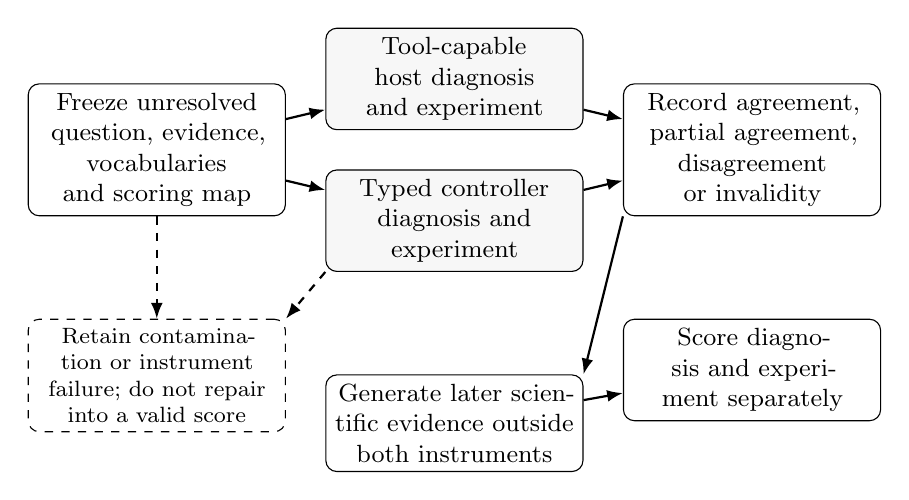
\begin{tikzpicture}[
  node distance=4mm and 5mm,
  box/.style={draw,rounded corners,align=center,text width=0.25\textwidth,minimum height=11mm,font=\small},
  decision/.style={draw,rounded corners,align=center,text width=0.25\textwidth,minimum height=12mm,font=\small,fill=black!3},
  bad/.style={draw,dashed,rounded corners,align=center,text width=0.25\textwidth,minimum height=10mm,font=\footnotesize},
  arrow/.style={-{Latex[length=2mm]},thick}
]
\node[box] (freeze) {Freeze unresolved question, evidence, vocabularies and scoring map};
\node[decision, right=of freeze, yshift=9mm] (host) {Tool-capable host diagnosis and experiment};
\node[decision, right=of freeze, yshift=-9mm] (ctrl) {Typed controller diagnosis and experiment};
\node[box, right=of host, yshift=-9mm] (relation) {Record agreement, partial agreement, disagreement or invalidity};
\node[bad, below=13mm of freeze] (fail) {Retain contamination or instrument failure; do not repair into a valid score};
\node[box, below=13mm of ctrl] (science) {Generate later scientific evidence outside both instruments};
\node[box, below=13mm of relation] (score) {Score diagnosis and experiment separately};
\draw[arrow] (freeze) -- (host);
\draw[arrow] (freeze) -- (ctrl);
\draw[arrow] (host) -- (relation);
\draw[arrow] (ctrl) -- (relation);
\draw[arrow] (relation.south west) -- (science.north east);
\draw[arrow] (science) -- (score);
\draw[arrow,dashed] (freeze.south) -- (fail.north);
\draw[arrow,dashed] (ctrl.south west) -- (fail.north east);
\end{tikzpicture}
\caption{Prospective dual-instrument lifecycle. The relation between the instruments is recorded before the later scientific result but does not validate either decision. Contamination and invalidity exit the valid series without being deleted.}
\label{fig:lifecycle}
\end{figure}

Immediately before each replacement freeze, the study checked whether an outcome-oriented scientific surface had become visible. Visibility was sufficient to retire the candidate even without opening that surface for scoring. This conservative rule sacrifices usable cases to protect the temporal meaning of ``prospective.''

\subsection{Deferred scoring}

The instruments never score themselves. A case-specific map states in advance what later observation would align with each diagnosis and which experiment would discriminate among the alternatives. A scientific result may align with a diagnosis, misalign with it, leave it unresolved or invalidate the item. The same result can simultaneously show that an experiment was appropriately chosen even when its motivating diagnosis was wrong.

The case series uses no pooled estimand. In particular, it does not compute the proportion of agreements, correct diagnoses or correct experiment choices. Those ratios would invite an unsupported interpretation as performance in a population of questions.

\section{Three prospectively frozen questions}

\subsection{Regime-characterization question}

The first question followed the failure of a compilation donor construction in a second coupling regime. The unresolved responsibility was whether the remaining gap required a new search, a new method language or explicit characterization of the representation regime. Both instruments selected regime characterization as the primary responsibility and an exact regime-membership computation as the next experiment. The typed controller also withheld a stronger representation change because its membership condition was not yet established.

Later work derived an exact regime predicate on the registered finite domains and closed the complementary support-two family on its registered domains. Under the frozen map, the diagnoses and experiment choices of both instruments are aligned. This result establishes one completed lifecycle only; it does not make regime characterization a generally reliable choice.

\subsection{Support-threshold stress-test question}

The second question concerned a proved sufficient region for a support-two representation. With objective weights $(t_{\mathrm{noncentral}},t_{\mathrm{central}},t_{\mathrm{tag}},t_{\mathrm{repeat}},\rho)$, the theorem applied when
\[
t_{\mathrm{central}}\geq 2t_{\mathrm{repeat}}
\quad\text{and}\quad
t_{\mathrm{noncentral}}\geq 2t_{\mathrm{repeat}}.
\]
The frozen point was $(4,3,2,2,0)$, one unit outside the first boundary and exactly on the second. Outside the sufficient region, the certificate was silent; it did not assert that support three was necessary.

Both instruments diagnosed the question as certificate silence with sharpness still open and selected an exact panel just outside the proved region. The later analysis compared unrestricted weighted optimization with exact support-at-most-two optimization on 53 frozen rows: three hostile one-object rows, two hostile two-object rows, 24 deterministic two-object rows and 24 deterministic three-object rows. It found zero rows in which unrestricted optimization improved on support two. An independent brute-force path also checked all three hostile one-object rows, and repeated executions produced identical scientific results.

The zero-gap observation follows the predeclared branch that aligns both diagnoses and both experiment choices. Its scope is the 53-row panel. It neither extends the all-size theorem nor establishes that support two remains sufficient everywhere outside the proved region. The sharpness question remains open.

\subsection{Reweighted-objective census question}

The third question changed the objective of a finite compilation family. Under the original objective, a proved boundary predicate characterized when the exact family matched a unary incumbent. The frozen alternative doubled the weight of selection cost while leaving preparation and width costs unchanged. The unary incumbent remained cheaper than the binary incumbent for every admitted nonzero instance, so the comparison stayed well defined.

Before any reweighted census existed, both instruments diagnosed the boundary predicate as objective-scoped and therefore expected that it would not transfer unchanged. Both selected the complete low-order reweighted census as the discriminating experiment. The diagnosis was plausible because the proof under the original objective contains coefficients affected by the changed selection weight.

The later census recomputed the exact family and compared the unchanged original predicate with the reweighted incumbent-equality label. It exhaustively covered
\[
729\ \text{ordered one-object cases}
\quad+\quad
38{,}760\ \text{reorder-quotiented two-object cases}
=39{,}489\ \text{cases}.
\]
It found zero predicate--label mismatches. There were no positive one-object cases under either definition and one positive two-object case under each. A second implementation path cross-checked 24 deterministic cases, and two complete census executions produced identical scientific results.

The frozen scoring map distinguished the branches. Any mismatch would have aligned most strongly with the selected objective-scoped diagnosis. Zero mismatches instead align, on the frozen finite domain, with structural invariance of the original predicate under this reweighting. Consequently, the diagnoses of both instruments are misaligned while their choice of the complete census is aligned. The result does not prove invariance at larger sizes, and the low-order domain is strongly label-imbalanced.

\section{Results}

Table~\ref{tab:cases} reports the complete valid series. No row is omitted and no aggregate rate is formed.

\begin{table}[t]
\centering
\caption{All valid prospectively frozen questions and bounded later observations.}
\label{tab:cases}
\small
\begin{tabularx}{\textwidth}{@{}p{0.10\textwidth}YYp{0.25\textwidth}@{}}
\toprule
Question & Frozen scientific question & Shared instrument decision & Later observation and scope \\
\midrule
Regime characterization & Which responsibility and experiment follow a cross-regime donor failure? & Characterize the representation regime; compute exact regime membership. & Exact finite-domain regime predicate and complementary support-two closure on registered domains. \\
Support-threshold stress test & Does a point just outside a proved support-two sufficient region expose a support-three need? & Treat the theorem as silent with sharpness open; run an exact near-boundary panel. & Zero unrestricted-versus-support-two gaps in 53 frozen rows; sharpness remains open. \\
Reweighted-objective census & Does an original boundary predicate change when selection cost is doubled? & Diagnose the predicate as objective-scoped; run the complete low-order census. & Zero predicate--label mismatches in 39,489 frozen cases; finite-domain diagnosis is misaligned and no larger-size theorem follows. \\
\bottomrule
\end{tabularx}
\end{table}

Table~\ref{tab:alignment} keeps agreement and deferred alignment separate. The third row is the headline counterexample: inter-instrument agreement coexists with two misaligned diagnoses.

\begin{table}[t]
\centering
\caption{Instrument relations and deferred alignment, reported by question rather than as rates.}
\label{tab:alignment}
\scriptsize
\begin{tabular}{@{}lcccccc@{}}
\toprule
& \multicolumn{2}{c}{Inter-instrument relation} & \multicolumn{2}{c}{Diagnostic alignment} & \multicolumn{2}{c}{Experiment alignment} \\
\cmidrule(lr){2-3}\cmidrule(lr){4-5}\cmidrule(l){6-7}
Question & diagnosis & experiment & Host & Controller & Host & Controller \\
\midrule
Regime characterization & agree & agree & \yes & \yes & \yes & \yes \\
Support-threshold stress test & agree & agree & \yes & \yes & \yes & \yes \\
Reweighted-objective census & agree & agree & \no & \no & \yes & \yes \\
\bottomrule
\end{tabular}
\end{table}

Three observations follow, each bounded by the row-wise design. First, the lifecycle can freeze heterogeneous decisions before the outcome and score them later. Second, agreement is not diagnostic validation. Third, diagnosis and experiment selection can separate: the reweighted-objective census was a productive choice precisely because it falsified the shared expectation on the frozen domain. The data do not show that experiment selection is generally more robust than diagnosis.

\section{Retained contamination and instrument limitations}

\subsection{Retired candidate questions}

The first planned expansion contained two other scientific questions. Before either pair of instrument outputs was frozen, outcome-oriented successor surfaces became visible. The study did not inspect those outcomes for scoring. Instead, both candidates were retired as contaminated, preserved in the audit history and replaced with scientifically distinct questions that were clean at freeze.

The two retired candidates are not part of the three valid cases and are not silently deleted. Their presence shows the cost of the prospective rule: potentially informative questions can become unusable when the scientific programme advances too quickly for an uncontaminated instrument freeze.

\subsection{Known fail-closed defects}

The frozen host instrument has two known failure modes. First, an outer capability envelope can indicate success while carrying semantically malformed content. The scientific parser can then fail without producing a typed disposition. Second, an immutable successful envelope can pin the deterministic request identity, preventing the ordinary failed-retry route.

These defects were not repaired between cases. Changing the instrument mid-series would create an instrument-version confound unless every case were prospectively repeated. Under the frozen rule, a malformed outcome-bearing case becomes instrument-invalid or cannot-check; the original content remains retained, and the case is not repaired in place into a valid score. Neither defect triggered in the three valid questions.

\begin{table}[t]
\centering
\caption{Protocol-retained events outside the valid three-question score.}
\label{tab:retained}
\small
\begin{tabularx}{\textwidth}{@{}p{0.25\textwidth}YY@{}}
\toprule
Event & Disposition & Scoring consequence \\
\midrule
Information-closure candidate & Outcome-oriented surface visible before instrument freeze. & Contaminated; retained and not retrospectively scored. \\
Enlarged-vocabulary candidate & Outcome-oriented surface visible before instrument freeze. & Contaminated; retained and not retrospectively scored. \\
Successful-envelope semantic malformation & Accepted unresolved defect of the frozen host. & If triggered after freeze, instrument-invalid or cannot-check; no in-place repair. \\
Immutable-success recovery obstruction & Accepted unresolved recoverability defect. & Original content retained; no ordinary failed-retry promotion into a valid score. \\
\bottomrule
\end{tabularx}
\end{table}

These are limitations, not positive results. Their inclusion prevents a favorable account that contains only clean agreements.

\section{Discussion}

\subsection{Agreement is a relation, not authority}

The central result is logical rather than statistical. In the reweighted-objective question, the host and controller used different decision machinery but shared the same research packet and conceptual vocabulary. Both inferred that reweighting the objective would change the boundary predicate. Their agreement did not introduce new evidence beyond those shared inputs. The later census did. Because the scoring map was fixed before the census, the zero-mismatch outcome could mark both diagnoses as misaligned without changing the earlier decisions.

This example cautions against promoting multi-agent consensus, repeated-model consistency or cross-instrument agreement into scientific correctness when the systems share evidence and framing. Agreement may still be useful as a descriptive variable in a larger study. It cannot serve as its own ground truth.

\subsection{Why experiment selection deserves a separate coordinate}

The reweighted-objective census also shows why evaluation should distinguish explanation from information acquisition. The instruments' diagnosis was wrong on the frozen domain, but their chosen census directly discriminated between the plausible hypotheses. Collapsing diagnosis and experiment into one success flag would either conceal the wrong explanation or discard the productive experiment.

This separation is compatible with decision-theoretic views of research planning, but the present evidence is only one observed separation. A future study could ask whether discriminating experiments remain useful more often than their motivating diagnoses remain correct. That question requires a larger prospectively sampled series and explicit cost accounting; it is not answered here.

\subsection{Contamination as data about the protocol}

The two retired candidates show that a prospective scientific benchmark interacts with the tempo of the research programme. A task can be well motivated and still cease to be admissible before execution. Recording that transition makes the selection process visible. Deleting contaminated candidates would hide one cost of the design and could bias a later account toward clean, easily frozen questions.

The same principle applies to instrument failures. A malformed-success event should not be interpreted as a scientific negative, but it should also not disappear. A fail-closed invalid or cannot-check state preserves the difference between absence of a scientific answer and evidence against a scientific hypothesis.

\subsection{Implication for research-agent evaluation}

The protocol is useful when agents participate in an evolving research process whose resolving evidence does not yet exist. It provides a way to evaluate the temporal decision rather than reconstruct a task retrospectively from a known outcome. The required elements are modest: a frozen question and evidence state, an explicit decision vocabulary, a deferred map, separate decision records and later evidence generated outside the evaluated instruments.

The present quantum-compilation cases establish feasibility under exact finite scientific analyses. Other fields may require different custody, uncertainty and scoring mechanisms. In empirical science, a later study might remain inconclusive; in such a case the deferred score should remain unresolved rather than being forced into alignment or misalignment.

\section{Limitations and unearned interpretations}

The strongest limitation is the study design. Three questions from one programme are neither random nor representative. They support a complete case-series statement and an explicit counterexample, but no reliability estimate, calibration curve, accuracy rate, confidence interval or population frequency.

The instruments share the scientific packet, upstream ontology and research history. The typed controller's observations and rule vocabulary are authored rather than naturally independent. The host and the people constructing the controller may also share conceptual priors. We claim heterogeneous execution paths, not statistical or causal independence.

The deferred outcomes are produced inside the same research programme. They are exact and independently replayed within their declared finite domains, but they are not external field-wide truth. The support-threshold stress test does not extend the all-size support-two theorem. The reweighted-objective census is exhaustive only for the declared one-object and two-object domains, and only one two-object case is positive. Zero mismatches do not prove a larger-size invariant.

The fail-closed policy is specified more strongly than it is stress-tested. The two known malformed-success and recovery defects did not trigger in the three valid cases. The study therefore does not establish general robustness, security or fault tolerance.

Finally, the cases do not compare the instruments with humans or with broader agent baselines. The paper makes no claim of autonomous discovery, superiority, governance readiness or transferable scientific judgment. A larger prospective reliability study is successor work and is not required to interpret the bounded counterexample reported here.

\section{Reproducibility, data and code availability}

The anonymous supplementary archive contains sanitized records for all three valid questions, both retired candidates, the frozen instrument relations, the deferred alignment fields and the bounded scientific outcomes. It also contains an independent verifier that reconstructs the three-row alignment table and checks the finite-domain arithmetic and the absence of aggregate performance fields. The archive deliberately omits identity-revealing custody material during double-blind review.

The sanitized records are offered under the Creative Commons Attribution 4.0 International licence and the verifier under the MIT licence. The exact provenance-bearing records and a permanent archival identifier will be released after the blind-review constraint is lifted and the human authors authorize the deposit. No personal, clinical or third-party restricted data are used.

\section{Ethics and broader-impact statement}

This work uses no human participants, animals, clinical records or personal data. Its primary integrity risks are authority laundering, selective reporting of clean agreements, retrospective scoring changes and hidden dependence between instruments. The protocol mitigates these risks by separating agreement from score, retaining contaminated and invalid events, and stating the dependence boundary. It does not eliminate misuse. The method should not be presented as proof that consensus is correct or that automated systems can govern scientific claims without human responsibility.

\section{Conclusion}

We reported a prospective three-question case series for decisions made before their scientific outcomes existed. A tool-capable host and a typed deterministic controller agreed on the diagnosis and experiment in every valid case. In one case, an exhaustive 39,489-case census showed that both shared diagnoses were misaligned on the frozen domain while both selected experiments were aligned. The case is a direct counterexample to agreement as diagnostic validation.

The result remains deliberately small. It establishes an executable measurement contract, one bounded counterexample, and a reason to score scientific diagnosis separately from experiment selection. It does not establish reliability, calibration, statistical independence, population rates or generalization. Larger prospective series belong to successor work; they do not change the interpretation of the complete three-row evidence reported here.

\bibliographystyle{tmlr}
\bibliography{references}

\end{document}
